% =====================================================================
%  Prabhavit Gupta, one-page CV (Doctolib - Software Engineer Java)
% =====================================================================
\documentclass[a4paper,10pt]{article}

\usepackage[T1]{fontenc}
\usepackage[utf8]{inputenc}
\usepackage[top=0.75cm,bottom=0.75cm,left=1.0cm,right=1.0cm]{geometry}
\usepackage{titlesec}
\usepackage{enumitem}
\usepackage{hyperref}
\usepackage{xcolor}
\usepackage{graphicx}

\definecolor{accent}{HTML}{1F4E78}
\hypersetup{colorlinks=true, urlcolor=accent, linkcolor=accent}
\pagestyle{empty}
\setlength{\parindent}{0pt}

\titleformat{\section}{\large\bfseries\color{accent}}{}{0em}{}[\vspace{-0.6em}\rule{\textwidth}{0.8pt}]
\titlespacing{\section}{0pt}{2pt}{1pt}

\newcommand{\role}[4]{%
 \textbf{#1} \hfill \textbf{#2}\\[1pt]%
 \textit{#3} \hfill \textit{#4}\\[2pt]%
}
\setlist[itemize]{leftmargin=1.2em, itemsep=0pt, topsep=1pt, parsep=0pt}

\begin{document}

% ================= HEADER =================
\begin{minipage}[c]{0.80\textwidth}
 {\Huge\bfseries Prabhavit Gupta}\\[3pt]
 {\color{accent}\large Software Engineer -- Backend \& Cloud Systems}\\[6pt]
 {\footnotesize +39 351 610 7807 ~$\vert$~
 \href{mailto:prabhavitg@gmail.com}{prabhavitg@gmail.com} ~$\vert$~
 \href{https://www.linkedin.com/in/prabhavit/}{linkedin.com/in/prabhavit} ~$\vert$~
 \href{https://github.com/prab-gupta}{github.com/prab-gupta} ~$\vert$~
 Venice / Milan, Italy}
\end{minipage}\hfill
\begin{minipage}[c]{0.18\textwidth}
 \raggedleft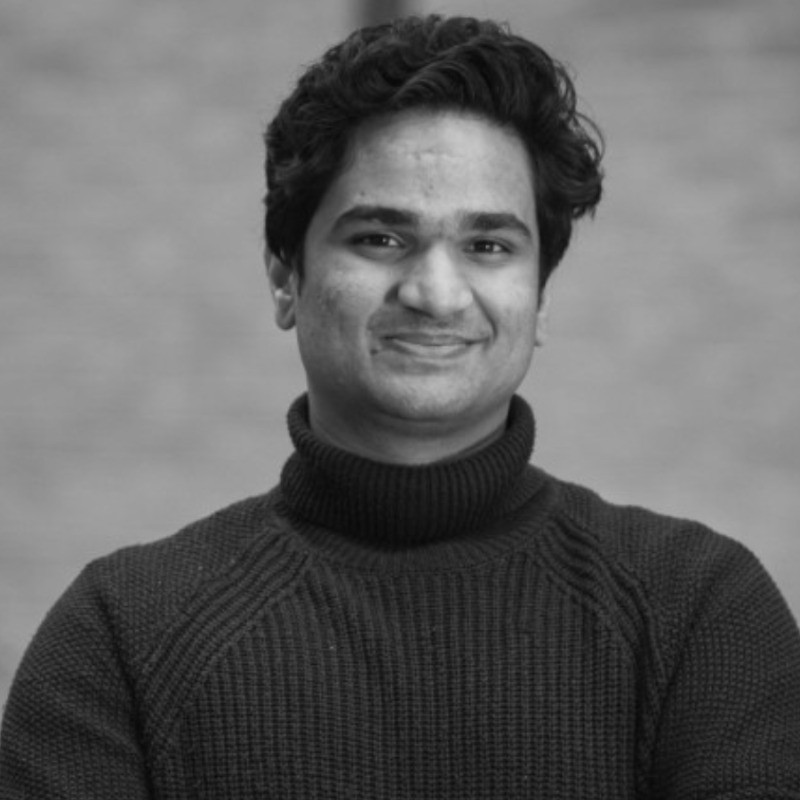
\includegraphics[width=2.0cm]{photo.jpg}
\end{minipage}
\vspace{-2pt}

% ================= SUMMARY =================
\section{Summary}
Product-minded Software Engineer with over 3 years of experience architecting and operating scalable, high-reliability microservices and SaaS platforms. Adept at applying object-oriented design and test-driven development (TDD) to build resilient APIs and data pipelines using PostgreSQL. Passionate about system reliability and integrating modern web technologies (JavaScript/TypeScript, HTML, CSS). Highly adaptable to Java, Kotlin, and .NET ecosystems, leveraging AI-powered development tools to accelerate learning, enforce engineering standards, and elevate code quality in fast-paced, cross-functional agile teams.

% ================= SKILLS =================
\section{Skills}
\begin{itemize}
 \item \textbf{Backend \& Architecture:} Microservices architecture, RESTful APIs, OOP principles, system reliability, transactional consistency, event-driven integrations
 \item \textbf{Languages \& Frameworks:} TypeScript, Node.js, Python, Object-Oriented paradigms (adaptable to Java/C\#), PHP (Laravel), Next.js, HTML, CSS, JavaScript
 \item \textbf{Cloud \& Infrastructure:} Cloud deployments (AWS), Docker, CI/CD, scalable SaaS architecture, uptime monitoring
 \item \textbf{Databases:} PostgreSQL, Supabase, database schema design, entity pipelines, strict schema validation
 \item \textbf{Engineering Practices:} Test-driven development (TDD), agile methodologies, AI-assisted coding for rapid feature iteration and root-cause analysis
\end{itemize}

% ================= EXPERIENCE =================
\section{Experience}

\role{\href{https://flowspace.co}{FlowSpace.co}}{Mar 2024 - Aug 2026}{Lead Developer \& Backend Engineer (Full-time, Freelance)}{London, UK (Remote)}
\begin{itemize}
 \item Led the core SaaS platform migration to a scalable architecture, designing resilient PostgreSQL database schemas and handling complex user data while scaling the user base from 2,000 to 4,500+.
 \item Engineered and operated production REST APIs integrating third-party platforms with robust schema validation, error handling, and uptime monitoring for high reliability.
 \item Implemented strict test-driven engineering standards and CI/CD pipelines, extensively leveraging AI-powered tools to accelerate delivery and ensure system health.
 \item Architected and deployed an end-to-end AI ingestion pipeline extracting structured data from unstructured multi-format sources, enforcing data integrity essential for enterprise applications.
\end{itemize}

\role{\href{https://ultrastrategy.com}{UltraStrategy.com}}{Dec 2024 - May 2025}{Backend Automation Developer (Collaborator)}{France (Remote)}
\begin{itemize}
 \item Developed a high-throughput data-processing pipeline using workflow automation and AI integrations, converting unstructured data into standardized relational schemas across diverse profiles.
\end{itemize}

\role{Urlink}{Apr 2025 - Jul 2025}{Project Manager \& AI-Assisted Developer (Freelance)}{Barcelona, Spain (Remote)}
\begin{itemize}
 \item Directed technical requirements and built backend application logic, database structures, and client automations with a strong focus on AI-assisted development tools and modern web tech.
\end{itemize}

\role{\href{https://get2germany.com}{Get2Germany.com}}{Jan 2024 - May 2024}{Backend Developer \& Automation Specialist (Part-time)}{Berlin, Germany (Remote)}
\begin{itemize}
 \item Built automated ETL pipelines integrating external APIs and custom workflows to aggregate, classify, and reliably serve complex domain data to front-end clients.
\end{itemize}

% ================= EDUCATION =================
\section{Education}
\textbf{Ca' Foscari University of Venice} \hfill Oct 2020 - Jun 2024\\
BA Philosophy, International Studies \& Economics (Minor: Entrepreneurship) \hfill Venice, Italy\\
{\footnotesize Core focus: Analytical logic, quantitative decision theory, economic modeling, and technology innovation.}

% ================= WORK AUTH =================
\vspace{2pt}
{\small \textbf{Work Authorization:} European Long Term Residence Permit (Italy); full Italian and EU work rights with zero sponsorship required. \quad \textbf{Languages:} English (fluent C2), Italian (conversational), Hindi (native).}

\end{document}
